\chapter{Future Work} \label{cha:future}

In this chapter, we will discuss improvements that can be made to this
implementation, and improvements that similar architecture should
consider.


\section{Testing}

We have highlighted the necessity of testing, especially in our architecture,
since we are maintaining the same \gls*{api}s, in different languages. We have
made some test data to ensure cohesion between these libraries, but this was
specially for translation between the different languages.

There should also be tests made to ensure that a module behaves the same, with
regard to the utility functionality offered by our libraries. This would help
in two areas.

Firstly, ensuring that we cover the same functionality across languages, as we
have not made the same module across different languages. We have three
different libraries, one for JavaScript modules, one for compile-time Rust
modules, and one for runtime Rust modules. So there might be differences in
these libraries.

Secondly, creating test data specially for utility functionalities would ensure
the provided utility functions work the same. An important example is the
optimization functions, covered in appendix \ref{app:a}. We need to ensure that
important core functionality works across libraries, as we do not want the
\gls*{ide} be tied to one solution.


\section{Language agnosticism improvements}

Steps should be made to mitigate the shortfall of this solution, with regard to
language agnosticism, especially with regard to module installation. The
differences in installation for \gls*{rsms} and \gls*{jsms} are mainly due to
how trivial it is to install JavaScript modules, compared to Rust modules.

A JavaScript module is installed once it is imported, while a Rust module needs
to be explicitly invoked. There are benefits in both scenarios.

For the JavaScript module, it is quite trivial to create an \textit{installer},
but more difficult to create testing applications for, as we can't properly
control module installation.

While for the Rust module, it is less trivial, for the module developer, since
they have to explicitly expose their module, and if they do not do it properly,
the Module will not be found. But it is quite trivial to create testing
applications, like the one that analyzed module dependencies, mentioned in
subsection \ref{ssec:mdv}.

\gls*{jsms} should enforce a similar system of module building as \gls*{rsms},
not only to ensure less semantic differences, but also to ensure safety, as
restricting the \gls*{jsms} is good.


\section{Attribute and instructions}

It is not possible to remove \textit{eventListener}s. The reason for this is due
to how event listeners are created. Since they send an event when they are
triggered, they need to have the event to send as an argument, and to remove
them from the \gls*{dom}, we need the same reference to the function. If we
want to remove them, we would have to require the module developer to pass the
exact same event they used to create the event listener, which could be
complicated.

A solution could be to store the created function, by mapping it to the event
name used in the creation, but what if the user has two events to send on a
button click, with the same name, but different arguments? How would that be
solved in a meaningful manner?


\section{Key presses}

A common feature of \gls*{ide}s is being able to have certain keybindings for
different actions. For example, in VS Code, one can hit \textit{CTRL}
$+$ \textit{n} to open up a new tab, with a new file. This system is not yet
possible in the \gls*{ide}.

Key-press registration could be introduced as a module, quite trivially. The
reason this was not done, was to not tempt our developer to spend all their time
creating a Vim module.


\section{Inconsistent UI representation}

Difficult to keep the \gls*{ui} representation consistent with the \gls*{dom}.
An example of this, is that the \gls*{ui} representation in the \gls*{ide} does
not store information like the possible \textit{value} an \gls{html} might
have. So for the editor module, there is no efficient way to know what text is
in the editor.

Another example, is for the module installer, there is no way for the module to
\textit{query} the \gls*{ui} for information about the form it presents the
user, seeing what values are in the fields. A workaround to this was used, where
depending on what element an \textit{eventListener} was added to, the sent event
would be \textit{sticky}, meaning it would add extra arguments to the
\textit{args} field of the event, like attribute information, id, value, etc.

But this would not update the \gls*{ui} stored in the \gls*{ide}, but rather
give modules a peek at the current \gls*{ui} state. A better solution would be
to somehow keep track of \textit{all} user interactions to the \gls*{dom}, and
somehow bubble these changes down to the backend, where the \gls*{ui}
representation is managed.


\section{Unify the tooling}

When a user wants to add a new module, regardless if its compile-time or
runtime, they have to specify what language the module they are adding.
Furthermore, if it is not a Rust module, extra information has to be added, to
ensure it is properly installed.


This is trivial to detect by a program. A user should be able to simply invoke
current installation tool with either a URL or a path to the module, and then
the tool can infer what kind of module it is, and add it to the configuration
file correctly.

This should also be integrated into the \gls*{ide}, but in a manner where the
different installers are modules themselves, which would enable other module
developers or maintainers to extend this functionality.

Similarly, other tooling, like generating the module dependency graph should be
integrated into the core. By using the Rust conditional compilation system, we
can conditionally include or exclude functionality, like these \gls*{cli} tools,
into the \gls*{ide}, allowing us to serve the \gls*{ide} without this
functionality if wanted.


\section{Modular editor}

The prototype editor module develop for this \gls*{ide} is subpar compared to
existing ones. A new one should be developed, in tandem with an \gls*{ls} client.
This development could of course happen after the new Magnolia compiler~\cite{wiig},
is stable, but regardless an \gls*{ls} client is needed. This would ensure that
this \gls*{ide} can support many languages.

The editor should then utilize existing technology that is already used by other
\gls*{ide}s, like the Tree-sitter\footnote{\url{https://github.com/tree-sitter/tree-sitter}}
parsing generator, which is used by, amongst others, Emacs.

The reason Tree-sitter is widely used, is that it supports incremental parsing,
allowing for real-time support, while the source code is being edited.


\subsection{Editor buffers}

One of the reasons the prototype editor module is subpar, is that it uses a
textarea \gls*{html}-element as input and renderer of text content. This should
be replaced by a buffer system, similar to how other \gls*{ide}s do. In the
figure \ref{fig:editorBuffer}, we can see a diagram of a module family which
enable a better, more modular, editor.

\begin{figure}
  \centering
  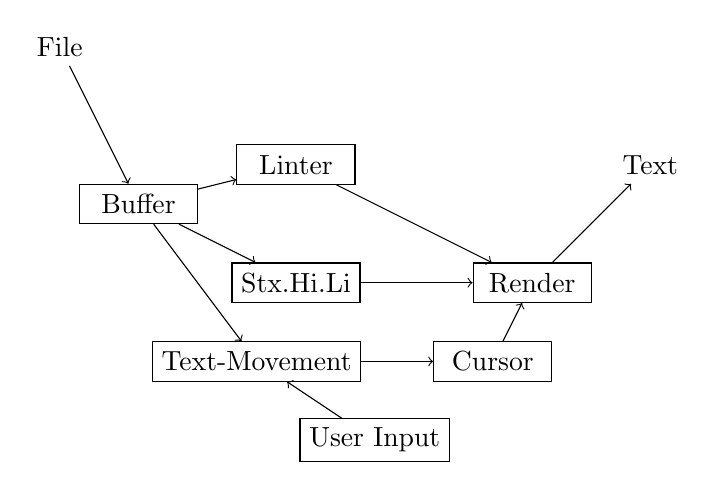
\begin{tikzpicture}
  % Nodes
  \node (file) [] at (-6, 3) {File};
  \node (parser) [rectangle, draw, minimum height=0.5cm, minimum width=1.5cm] at (-5, 1) {Buffer};
  \node (stxhili) [rectangle, draw, minimum height=0.5cm, minimum width=1.5cm] at (-3, 0) {Stx.Hi.Li};
  \node (text-movement) [rectangle, draw, minimum height=0.5cm, minimum width=1.5cm] at (-3.5, -1) {Text-Movement};
  \node (linter) [rectangle, draw, minimum height=0.5cm, minimum width=1.5cm] at (-3, 1.5) {Linter};
  \node (cursor) [rectangle, draw, minimum height=0.5cm, minimum width=1.5cm] at (-0.5, -1) {Cursor};
  \node (user-input) [rectangle, draw, minimum height=0.5cm, minimum width=1.5cm] at (-2, -2) {User Input};
  \node (render) [rectangle, draw, minimum height=0.5cm, minimum width=1.5cm] at (0, 0) {Render};
  \node (text) at (1.5, 1.5) {Text};
  % Arrow
  \draw[->] (file) -- (parser) node[midway, above] {};
  \draw[->] (parser) -- (stxhili) node[midway, above] {};
  \draw[->] (parser) -- (linter) node[midway, above] {};
  \draw[->] (parser) -- (text-movement) node[midway, above] {};
  \draw[<-] (render) -- (stxhili) node[midway, above] {};
  \draw[<-] (render) -- (linter) node[midway, above] {};
  \draw[<-] (cursor) -- (text-movement) node[midway, above] {};
  \draw[<-] (text-movement) -- (user-input) node[midway, above] {};
  \draw[->] (cursor) -- (render) node[midway, above] {};
  \draw[->] (render) -- (text) node[midway, above] {};
\end{tikzpicture}


  \caption{
    Diagram of a module dependency graph for an editor module family. The
    contents of a file are stored in a buffer, which different modules, linter,
    syntax highlighting and text movement, can handle the text in their
    respective format.
  }
  \label{fig:editorBuffer}
\end{figure}

The general idea is for a buffer to contain the contents of a file. The final
step is for some render module to transform the text into some \gls*{html} that
is actually rendered by the \gls*{ide} to the user. The linter and syntax
highlighter modules add colour to keywords, depending on what language the file
is written in, while the linter adds indications to a user if what they have
written is incorrect, if there is a warning or error. Both of which could
utilize Tree-sitter.

Given that files are just a long string of bytes, some cursor module is needed,
to keep track of where the user is inserting text. This also allows for other
modules, like, for example a text movement module to register user key presses
as text movement.


\section{Improvements to the module architecture}

Other popular \gls*{ide}s have a form of module architecture. For instance, in
NetBeans, modules can directly invoke methods of other modules. This is due to
the modules being written in the same language, and can have the same underlying
\gls*{abi}.

We circumvented this issue, by having our \gls*{ide} be the intermediary, but
this restrictions means we can only indirectly invoke the methods of other
modules. An improvement to this architecture, would be for modules to directly
interact with each other, and for the \gls*{ide} itself to be entirely made out
of modules, the only thing the \textit{core} of the zero-core does, is
initialized modules. Letting modules be in charge of their own cycles, when to
be invoked, who to invoke, etc.
